% ---------------------------------------------------------------
% Generated by FlowTikZ (flowcharts and data charts to LaTeX)
% Every coordinate below is derived from the editor diagram model.
% Safe to edit by hand, but regenerating will overwrite changes.
% ---------------------------------------------------------------

\documentclass[border=8pt]{standalone}
\usepackage[T1]{fontenc}
\usepackage[utf8]{inputenc}
\usepackage{amsmath}
\usepackage{amssymb}
\usepackage{xcolor}
\usepackage{tikz}
\usepackage[version=4]{mhchem}
\usepackage{chemfig}

% ---- Colour definitions ----
\definecolor{fc12161C}{HTML}{12161C}
\definecolor{fc1F2933}{HTML}{1F2933}

% ---- Style definitions ----
\tikzset{
  fcnode/.style={
    draw, inner sep=0pt, outer sep=0pt, align=center,
    line join=round, line cap=butt
  },
  fcpath/.style={line join=round, line cap=butt},
  fcedge/.style={line join=round, line cap=butt},
  fclabel/.style={inner sep=1.4pt, outer sep=0pt, align=center},
}
\tikzset{fcformula/.style={inner sep=0pt, outer sep=0pt}}

\begin{document}
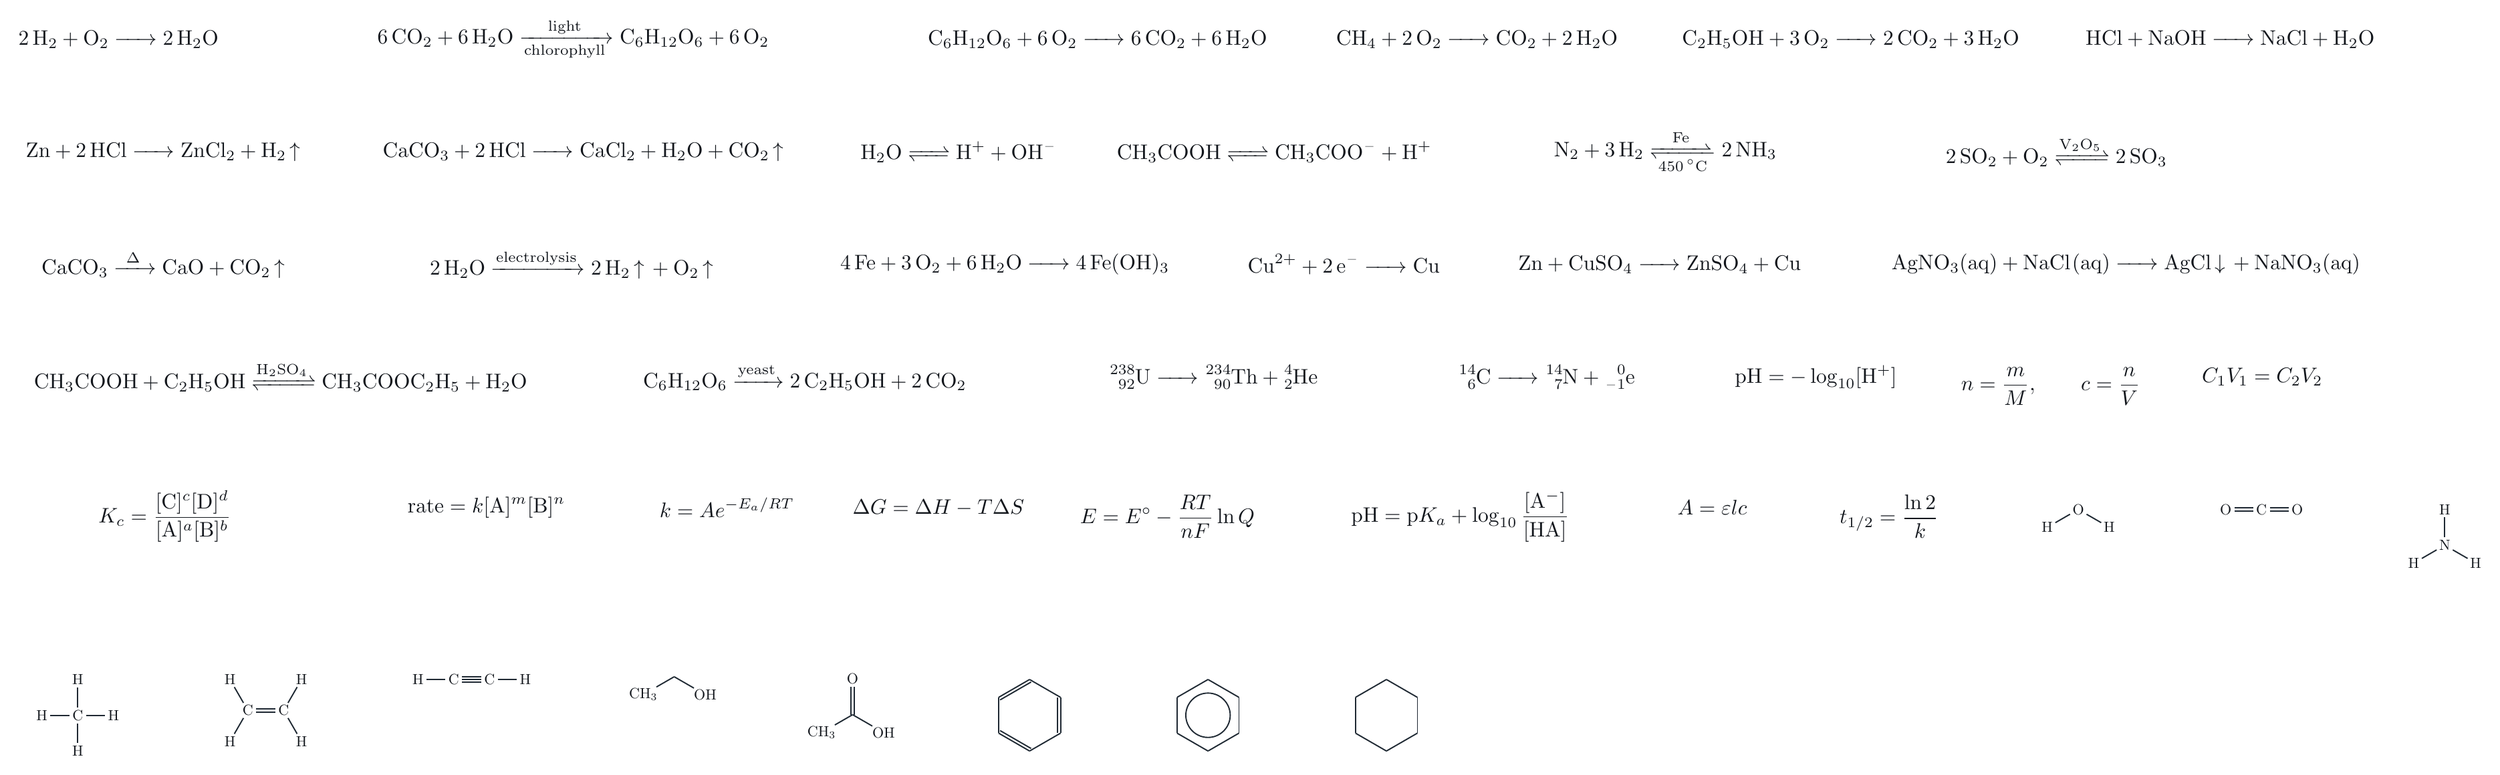
\begin{tikzpicture}[x=1cm, y=1cm]
  % ---- Nodes ----
  % g1 - Chemical formula "2H2 + O2 -> 2H2O"
  \node[fcformula, scale=1.138, text=fc12161C] (g1) at (3.76,-2.27) {\ce{2H2 + O2 -> 2H2O}};
  % g2 - Chemical formula "6CO2 + 6H2O ->[light][chlorophyll] C6H12O6 + 6O2"
  \node[fcformula, scale=1.138, text=fc12161C]
        (g2) at (12.4,-2.27) {\ce{6CO2 + 6H2O ->[light][chlorophyll] C6H12O6 + 6O2}};
  % g3 - Chemical formula "C6H12O6 + 6O2 -> 6CO2 + 6H2O"
  \node[fcformula, scale=1.138, text=fc12161C]
        (g3) at (22.36,-2.27) {\ce{C6H12O6 + 6O2 -> 6CO2 + 6H2O}};
  % g4 - Chemical formula "CH4 + 2O2 -> CO2 + 2H2O"
  \node[fcformula, scale=1.138, text=fc12161C]
        (g4) at (29.57,-2.27) {\ce{CH4 + 2O2 -> CO2 + 2H2O}};
  % g5 - Chemical formula "C2H5OH + 3O2 -> 2CO2 + 3H2O"
  \node[fcformula, scale=1.138, text=fc12161C]
        (g5) at (36.67,-2.27) {\ce{C2H5OH + 3O2 -> 2CO2 + 3H2O}};
  % g6 - Chemical formula "HCl + NaOH -> NaCl + H2O"
  \node[fcformula, scale=1.138, text=fc12161C]
        (g6) at (43.88,-2.27) {\ce{HCl + NaOH -> NaCl + H2O}};
  % g7 - Chemical formula "Zn + 2HCl -> ZnCl2 + H2 ^"
  \node[fcformula, scale=1.138, text=fc12161C]
        (g7) at (4.64,-4.41) {\ce{Zn + 2HCl -> ZnCl2 + H2 ^}};
  % g8 - Chemical formula "CaCO3 + 2HCl -> CaCl2 + H2O + CO2 ^"
  \node[fcformula, scale=1.138, text=fc12161C]
        (g8) at (12.62,-4.41) {\ce{CaCO3 + 2HCl -> CaCl2 + H2O + CO2 ^}};
  % g9 - Chemical formula "H2O <=> H+ + OH-"
  \node[fcformula, scale=1.138, text=fc12161C] (g9) at (19.72,-4.41) {\ce{H2O <=> H+ + OH-}};
  % g10 - Chemical formula "CH3COOH <=> CH3COO- + H+"
  \node[fcformula, scale=1.138, text=fc12161C]
        (g10) at (25.72,-4.41) {\ce{CH3COOH <=> CH3COO- + H+}};
  % g11 - Chemical formula "N2 + 3H2 <=>[Fe][450 $^\circ$C] 2NH3"
  \node[fcformula, scale=1.138, text=fc12161C]
        (g11) at (33.15,-4.41) {\ce{N2 + 3H2 <=>[Fe][450 $^\circ$C] 2NH3}};
  % g12 - Chemical formula "2SO2 + O2 <=>[V2O5] 2SO3"
  \node[fcformula, scale=1.138, text=fc12161C]
        (g12) at (40.58,-4.41) {\ce{2SO2 + O2 <=>[V2O5] 2SO3}};
  % g13 - Chemical formula "CaCO3 ->[$\Delta$] CaO + CO2 ^"
  \node[fcformula, scale=1.138, text=fc12161C]
        (g13) at (4.64,-6.55) {\ce{CaCO3 ->[$\Delta$] CaO + CO2 ^}};
  % g14 - Chemical formula "2H2O ->[electrolysis] 2H2 ^ + O2 ^"
  \node[fcformula, scale=1.138, text=fc12161C]
        (g14) at (12.4,-6.55) {\ce{2H2O ->[electrolysis] 2H2 ^ + O2 ^}};
  % g15 - Chemical formula "4Fe + 3O2 + 6H2O -> 4Fe(OH)3"
  \node[fcformula, scale=1.138, text=fc12161C]
        (g15) at (20.6,-6.55) {\ce{4Fe + 3O2 + 6H2O -> 4Fe(OH)3}};
  % g16 - Chemical formula "Cu^2+ + 2e- -> Cu"
  \node[fcformula, scale=1.138, text=fc12161C]
        (g16) at (27.04,-6.55) {\ce{Cu^2+ + 2e- -> Cu}};
  % g17 - Chemical formula "Zn + CuSO4 -> ZnSO4 + Cu"
  \node[fcformula, scale=1.138, text=fc12161C]
        (g17) at (33.04,-6.55) {\ce{Zn + CuSO4 -> ZnSO4 + Cu}};
  % g18 - Chemical formula "AgNO3(aq) + NaCl(aq) -> AgCl v + NaNO3(aq)"
  \node[fcformula, scale=1.138, text=fc12161C]
        (g18) at (41.9,-6.55) {\ce{AgNO3(aq) + NaCl(aq) -> AgCl v + NaNO3(aq)}};
  % g19 - Chemical formula "CH3COOH + C2H5OH <=>[H2SO4] CH3COOC2H5 + H2O"
  \node[fcformula, scale=1.138, text=fc12161C]
        (g19) at (6.84,-8.69) {\ce{CH3COOH + C2H5OH <=>[H2SO4] CH3COOC2H5 + H2O}};
  % g20 - Chemical formula "C6H12O6 ->[yeast] 2C2H5OH + 2CO2"
  \node[fcformula, scale=1.138, text=fc12161C]
        (g20) at (16.8,-8.69) {\ce{C6H12O6 ->[yeast] 2C2H5OH + 2CO2}};
  % g21 - Chemical formula "^{238}_{92}U -> ^{234}_{90}Th + ^{4}_{2}He"
  \node[fcformula, scale=1.138, text=fc12161C]
        (g21) at (24.56,-8.69) {\ce{^{238}_{92}U -> ^{234}_{90}Th + ^{4}_{2}He}};
  % g22 - Chemical formula "^{14}_{6}C -> ^{14}_{7}N + ^{0}_{-1}e"
  \node[fcformula, scale=1.138, text=fc12161C]
        (g22) at (30.89,-8.69) {\ce{^{14}_{6}C -> ^{14}_{7}N + ^{0}_{-1}e}};
  % g23 - Formula "\mathrm{pH}=-\log_{10}[\mathrm{H^{+}}]"
  \node[fcformula, scale=1.138, text=fc12161C]
        (g23) at (36.01,-8.69) {$\displaystyle \mathrm{pH}=-\log_{10}[\mathrm{H^{+}}]$};
  % g24 - Formula "n=\frac{m}{M},\qquad c=\frac{n}{V}"
  \node[fcformula, scale=1.138, text=fc12161C]
        (g24) at (40.47,-8.86) {$\displaystyle n=\frac{m}{M},\qquad c=\frac{n}{V}$};
  % g25 - Formula "C_{1}V_{1}=C_{2}V_{2}"
  \node[fcformula, scale=1.138, text=fc12161C]
        (g25) at (44.49,-8.69) {$\displaystyle C_{1}V_{1}=C_{2}V_{2}$};
  % g26 - Formula "K_{c}=\frac{[\mathrm{C}]^{c}[\mathrm{D}]^{d}}{[\"
  \node[fcformula, scale=1.138, text=fc12161C]
        (g26) at (4.64,-11.34) {$\displaystyle K_{c}=\frac{[\mathrm{C}]^{c}[\mathrm{D}]^{d}}{[\mathrm{A}]^{a}[\mathrm{B}]^{b}}$};
  % g27 - Formula "\text{rate}=k[\mathrm{A}]^{m}[\mathrm{B}]^{n}"
  \node[fcformula, scale=1.138, text=fc12161C]
        (g27) at (10.75,-11.17) {$\displaystyle \text{rate}=k[\mathrm{A}]^{m}[\mathrm{B}]^{n}$};
  % g28 - Formula "k=Ae^{-E_{a}/RT}"
  \node[fcformula, scale=1.138, text=fc12161C]
        (g28) at (15.32,-11.17) {$\displaystyle k=Ae^{-E_{a}/RT}$};
  % g29 - Formula "\Delta G=\Delta H-T\Delta S"
  \node[fcformula, scale=1.138, text=fc12161C]
        (g29) at (19.34,-11.17) {$\displaystyle \Delta G=\Delta H-T\Delta S$};
  % g30 - Formula "E=E^{\circ}-\frac{RT}{nF}\ln Q"
  \node[fcformula, scale=1.138, text=fc12161C]
        (g30) at (23.69,-11.34) {$\displaystyle E=E^{\circ}-\frac{RT}{nF}\ln Q$};
  % g31 - Formula "\mathrm{pH}=\mathrm{p}K_{a}+\log_{10}\frac{[\mat"
  \node[fcformula, scale=1.138, text=fc12161C]
        (g31) at (29.25,-11.34) {$\displaystyle \mathrm{pH}=\mathrm{p}K_{a}+\log_{10}\frac{[\mathrm{A^{-}}]}{[\mathrm{HA}]}$};
  % g32 - Formula "A=\varepsilon lc"
  \node[fcformula, scale=1.138, text=fc12161C]
        (g32) at (34.04,-11.17) {$\displaystyle A=\varepsilon lc$};
  % g33 - Formula "t_{1/2}=\frac{\ln 2}{k}"
  \node[fcformula, scale=1.138, text=fc12161C]
        (g33) at (37.4,-11.34) {$\displaystyle t_{1/2}=\frac{\ln 2}{k}$};
  % g34 - Molecule "3 atoms"
  \node[fcformula] (g34) at (40.9949,-11.376) {%
    \scalebox{0.797}{\color{fc12161C}\setchemfig{atom sep=0.853cm, bond style={draw=fc1F2933, line width=0.857pt}}\chemfig{{O}(-[:210]{H})-[:330]{H}}}};
  % g35 - Molecule "3 atoms"
  \node[fcformula] (g35) at (44.4758,-11.206) {%
    \scalebox{0.797}{\color{fc12161C}\setchemfig{atom sep=0.853cm, bond style={draw=fc1F2933, line width=0.857pt}}\chemfig{{O}=[:0]{C}=[:0]{O}}}};
  % g36 - Molecule "4 atoms"
  \node[fcformula] (g36) at (47.9567,-11.716) {%
    \scalebox{0.797}{\color{fc12161C}\setchemfig{atom sep=0.853cm, bond style={draw=fc1F2933, line width=0.857pt}}\chemfig{{N}(-[:210]{H})(-[:330]{H})-[:90]{H}}}};
  % g37 - Molecule "5 atoms"
  \node[fcformula] (g37) at (2.986,-15.118) {%
    \scalebox{0.797}{\color{fc12161C}\setchemfig{atom sep=0.853cm, bond style={draw=fc1F2933, line width=0.857pt}}\chemfig{{C}(-[:90]{H})(-[:0]{H})(-[:270]{H})-[:180]{H}}}};
  % g38 - Molecule "6 atoms"
  \node[fcformula] (g38) at (6.558,-15.0269) {%
    \scalebox{0.797}{\color{fc12161C}\setchemfig{atom sep=0.853cm, bond style={draw=fc1F2933, line width=0.857pt}}\chemfig{{C}(=[:0]{C}(-[:60]{H})-[:300]{H})(-[:120]{H})-[:240]{H}}}};
  % g39 - Molecule "4 atoms"
  \node[fcformula] (g39) at (10.47,-14.438) {%
    \scalebox{0.797}{\color{fc12161C}\setchemfig{atom sep=0.853cm, bond style={draw=fc1F2933, line width=0.857pt}}\chemfig{{H}-[:0]{C}~[:0]{C}-[:0]{H}}}};
  % g40 - Molecule "3 atoms"
  \node[fcformula] (g40) at (14.2909,-14.608) {%
    \scalebox{0.797}{\color{fc12161C}\setchemfig{atom sep=0.853cm, bond style={draw=fc1F2933, line width=0.857pt}}\chemfig{{CH_3}-[:30]-[:330]{OH}}}};
  % g41 - Molecule "4 atoms"
  \node[fcformula] (g41) at (17.6807,-14.948) {%
    \scalebox{0.797}{\color{fc12161C}\setchemfig{atom sep=0.853cm, bond style={draw=fc1F2933, line width=0.857pt}}\chemfig{{CH_3}-[:30](=[:90]{O})-[:330]{OH}}}};
  % g42 - Molecule "6 atoms"
  \node[fcformula] (g42) at (21.0705,-15.118) {%
    \scalebox{0.797}{\color{fc12161C}\setchemfig{atom sep=0.853cm, bond style={draw=fc1F2933, line width=0.857pt}}\chemfig{?[a]=^[:210]-[:270]=^[:330]-[:30]=^[:90]?[a,{-}]}}};
  % g43 - Molecule "6 atoms"
  \node[fcformula] (g43) at (24.4603,-15.118) {%
    \scalebox{0.797}{\color{fc12161C}\setchemfig{atom sep=0.853cm, bond style={draw=fc1F2933, line width=0.857pt}}\chemfig{?[a](-[:270,1,,,draw=none]{\tikz{\draw[draw=fc1F2933,line width=0.857pt] (0,0) circle (0.5289);}})-[:210]-[:270]-[:330]-[:30]-[:90]?[a,{-}]}}};
  % g44 - Molecule "6 atoms"
  \node[fcformula] (g44) at (27.8501,-15.118) {%
    \scalebox{0.797}{\color{fc12161C}\setchemfig{atom sep=0.853cm, bond style={draw=fc1F2933, line width=0.857pt}}\chemfig{?[a]-[:210]-[:270]-[:330]-[:30]-[:90]?[a,{-}]}}};
\end{tikzpicture}
\end{document}